% !TEX TS-program = pdflatex
% !TEX encoding = UTF-8 Unicode

% This file is a template using the "beamer" package to create slides for a talk or presentation

\documentclass{beamer}


\mode<presentation>
{
	%%%%%%%%%%%%%%%%%%% use this theme %%%%%%%%%%%%%%%%%%%
  %\usetheme{Warsaw}
  % or ...

  \setbeamercovered{transparent}
  % or whatever (possibly just delete it)
}


\addtobeamertemplate{navigation symbols}{}{%
    \usebeamerfont{footline}%
    \usebeamercolor[fg]{footline}%
    \hspace{1em}%
    \insertframenumber/\inserttotalframenumber
}

\usepackage[english]{babel}
\usepackage{amssymb, amsmath}
% or whatever
\usepackage{graphicx}
\usepackage{subcaption}
\usepackage[utf8]{inputenc}
\usepackage{hyperref}
% or whatever

\usepackage{amsfonts} 
\usepackage{array}

\newenvironment{conditions}
  {\par\vspace{\abovedisplayskip}\noindent\begin{tabular}{>{$}l<{$} @{${}={}$} l}}
  {\end{tabular}\par\vspace{\belowdisplayskip}}
  
  
\newenvironment{conditions2}
  {\par\vspace{\abovedisplayskip}\noindent\begin{tabular}{>{$}l<{$} @{${}{}$} l}}
  {\end{tabular}\par\vspace{\belowdisplayskip}}
  
  
\title[Implicit Preferences] % (optional, use only with long paper titles)
{Epidemiological Modelling of Coronavirus Infection in Quarantined Population}

\subtitle
{A Outline of Project for MATH371 Wi2020}

\author[natasha]{Natasha Ting\\[5mm]{\footnotesize Instructor: Prof Jay Newby}}
%\author[] % (optional, use only with lots of authors)
%{Natasha Ting\inst{} \and %\inst{2}
%}
% - Give the names in the same order as the appear in the paper.
% - Use the \inst{?} command only if the authors have different
%   affiliation.

\institute[University of Alberta] % (optional, but mostly needed)
{
  \inst{}%
  Department of Mathematical and Statistical Sciences\\
  University of Alberta
%  \and
 % \inst{2}%
 % Department of Theoretical Philosophy\\
 % University of Elsewhere
 }
 \date{2020}
% - Use the \inst command only if there are several affiliations.
% - Keep it simple, no one is interested in your street address.

{}
\subject{Search and Match, Implicit Preferences}

\pagenumbering{roman}
\begin{document}
\begin{frame}
  \titlepage
\end{frame}

\begin{frame}{Outline}
  \tableofcontents
  % You might wish to add the option [pausesections]
\end{frame}


\section{Motivation and Objective}

\begin{frame}{Objective}
	\begin{itemize}
	\item to explore the SIRD model and its stability points
	\item to estimate parameters of the SIR model given COVID-19 epidemiological data from Wuhan of China, Italy, and Canada
	\item to explore SIRD models that embed age compartments, and quarantining of population
	\end{itemize}
\end{frame}

\subsection{Motivation: COVID-19}
\begin{frame}{COVID-19}
	COVID-19 is caused by a novel virus named SARS-CoV-2 that found its first confirmed case in December 2020. By March 2020, $780,000$ cases of COVID-19 have been confirmed around the world, and it is still developing. \\
\end{frame}

%%%%%%%%%%%%% Not ready to include literature review yet %%%%%%%%%%%%

%\subsection{Previous Work}

%\begin{frame}{Make Titles Informative.}
%\end{frame}

%\begin{frame}{Make Titles Informative.}
%\end{frame}

%%%%%%%%%%%%%%%%%%%%%%%%%%%%%%%%%%%%%%%%%%%%%%%%

\section{The Models}
\subsection{SIRD}
\begin{frame}{SIRD Model}
The fraction of individuals susceptible to contract COVID-19 in a population , $\frac{S}{N} = s$, fraction of infected individuals, $\frac{I}{N} = i$, fraction of removed individuals, $\frac{R}{N} = r$ and fraction of dead, $\frac{D}{N} = d$ change in dynamic described in the following planar system: 
\begin{equation}
       \begin{array}{ll}
      \dot{s} = - \beta s i  & \quad s(0) = s_0 \\
       \dot{i} = \beta s i - (\alpha + \mu)i & \quad i(0) = i_0 \\
       \dot{r} = \alpha i  & \quad r(0) = r_0 \\ 
       \dot{d} = \mu i & \quad d(0) = 0 
        \end{array}
\end{equation}
where:
\begin{conditions}
\beta & infection rate; \quad \quad $\frac{1}{\beta}$ = average days to be infected \\
\alpha & recovery rate; \quad \quad $\frac{1}{\alpha}$ = average days to recover \\
\mu & death rate \\
R_0 & basic reproduction number, the avg number infected by 1 person \\
\end{conditions}
\end{frame}

\begin{frame}{Stability Analysis of the SIRD}
	Taking out $d = 1 - s - i - d $, the planar system in (1) can be rewritten as $$\mathbf{\dot{x}} = \mathbf{F}(\mathbf{x})$$ 
	where $\mathbf{x}^{T} = [s \;\;i\;\; r]$ \\
	at steady state (ss), $\mathbf(\dot{x}) = 0 \implies $ $$\mathbf{x} = \hat{\mathbf{x}} = \begin{pmatrix} s_{ss} \\ 0 \\ r \end{pmatrix}$$ 
	with Jacobian matrix $$J{\mathbf{\hat{x}}} = \begin{pmatrix} 0 & \beta s_{ss} & 0\\ 0 & \beta s_{ss} - (\alpha + \mu) & 0 \\ 0 & \alpha & 0  \end{pmatrix} $$ and eigenvalues $\lambda_1, \lambda_2 = 0, \lambda_3 = bs - (\alpha + \mu) <0 $ since $s_{ss} < s_{I_{max}}$
	
\end{frame}

\begin{frame}{Phase Plane Analysis}
\begin{figure}
  \includegraphics[width=7cm,height=7cm,keepaspectratio]{phaseplane.png}
  \caption{Phase plane plot obtained from Jay Newby 2020 lecture materials}
  \label{fig:phaseplan}
\end{figure}
\vspace{-6mm}
The phase plane plot reveals that $i = 0$, $s = 0$ is a stable point. 
\end{frame}


\subsection{SIR with Quarantine}
\begin{frame}{SIR with Quarantine}
The SIR model with quarantine adds a compartment $\dot{q} = \frac{Q}{N}$, where $Q$ represents the quarantined infected individuals. Infected individuals are quarantined at rate $\gamma$, recover at rate $\alpha$, and perish at rate $\mu$.   
\begin{equation}
       \begin{array}{ll}
      \dot{s} = - \beta s i  & \quad s(0) = s_0 \\
       \dot{i} = \beta s i - (\alpha + \mu)i & \quad i(0) = i_0 \\
       \dot{r} = \alpha i  & \quad r(0) = r_0 \\ 
       \dot{q} = \gamma i - \mu q - \alpha q & \quad q(0) = 0 \\
       \dot{d} = \mu i & \quad d(0) = 0 
        \end{array}
\end{equation}
\end{frame}


\section{Assumptions}
\begin{frame}{Assumptions}
The SIR family of models assume:
\begin{itemize}
	\item instantaneous infection, recovery of individuals
	\item no delay in any effect, including death
\end{itemize}
which is not captured in the publicly available data collected by the health authority. \\

\bigskip 
In addition, while the solutions to the SIR model is unique, the optimal parameters found by equation (3) takes different values given different initial guess fed to the solver. 

\end{frame}


%%%%%%%%%%%%%%%%%%%%%%%%%%%%%%%%%%%%%%%%

\section{Methods of Estimation}

\subsection{Least-square (Plateaued)}
\begin{frame}{Minimisation Problem (Plateaued)}

To estimate parameters from data from regions that \textbf{have reached} a plateau-ing trend in the number of confirmed cases (infected), we solve the following problem: 

\begin{equation}
\begin{aligned}
& \underset{\alpha, \beta=1, \mu, N}{\text{minimize}} & &  \left(\frac{I_{max} - \widehat{I}_{max}}{I_{max}}\right)^2 + \frac{1}{T} \sum_{t=1}^{T} \left(\frac{R_t - \widehat{R_t}}{R_{max}}\right)^2 + \left(\frac{D_t - \widehat{D_t}}{D_{max}}\right)^2\\
& \text{subject to}
& & 0 \leq \frac{\alpha + \mu}{\beta} \leq \left(\frac{N-( I + R + D )}{N} \right)\bigg\rvert_{I=I_{max}}
 \end{aligned}
\end{equation}
\end{frame}

\begin{frame}{For Non-Plateaued Data}
For data from regions that have not reached the plateauing stage of the data, we solve the following minimisation problem for each compartment $i, r, d$. \\ 
I.e. assuming $s = 1$, for $i$: \\
\begin{equation}
\begin{aligned}
& \underset{i_0, k_0}{\text{minimize}} & &  E = \sum_{t=1}^{T} (i_t - \widehat{i_t})^2 \\
& \text{subject to}
& & \hat{i} = i_0 e^{k_0 i} \\
& \text{where } k = \beta -\alpha - \mu &
 \end{aligned}
\end{equation}
\end{frame}


\begin{frame}{For Non-Plateaued Data}
From Eq(4) we get
\begin{equation}
\begin{aligned}
& \hat{i} = i_0 e^{k_0 t} \\
& \hat{r} = r_0 e^{k_0 t} \\
& \hat{d} = d_0 e^{k_0 t} 
 \end{aligned}
\end{equation}
In addition, $$r_0 = \frac{i_0 \alpha}{k_0}, \quad d_0 = \frac{i_0 \mu}{k_0} $$
$$\implies \alpha = \frac{r_0 k_0}{ i_0}, \quad \mu = \frac{d_0 k_0}{ i_0} $$
$$\implies \beta = k_0 + \frac{k_0}{i_0} (d_0 + r_0)$$

\end{frame}


\subsection{Time Scale Matching}
\begin{frame}{Time Scale of Estimated Data}
Using Euler’s method, a differential form $\dot{s}=-\beta si$ can be expressed as
	$$s_{t+1} = s_t + dt (-\beta s_t i_t)$$
Which we consider as 
	$$s_{t+1} = s_t + \beta dt (- s_t i_t)$$
Thus, a change in $\beta$ leads to a change in the timescale. In Eq(3) we assumed $\beta$ = 1. \\
\end{frame}

\begin{frame}{The Time-scale constant}
The estimated data has time scale $t'$. It is scaled to match the timescale used by the data in $t$ time scale. We obtain 
\begin{equation}k = \frac{t_m}{t'_m} \end{equation} 
where $t_m $ is the time at which $i(t)$ is maximum and  $t'_m$ is the time when $\hat{i}(t')$ is maximum. 
\bigskip
\\
Eq (6) implies $t' = \frac{t}{k}$. Thus, to match timescales, $\hat{s}(t') = \hat{s}(\frac{t}{k}) $. \\ 
In addition, since $\beta = 1$ in Eq(3), the estimated parameters are scaled i.e. 
$$\alpha = \frac{\hat{\alpha}}{k}, \beta = \frac{1}{k}, \mu = \frac{\hat{\mu}}{k}, N = \hat{N}$$.
\end{frame}

\section{Result}
\begin{frame}{Result}

The estimated parameters depends on the initial conditions fed to the optimization algorithm. 

\end{frame}

\begin{frame}
\begin{figure}
  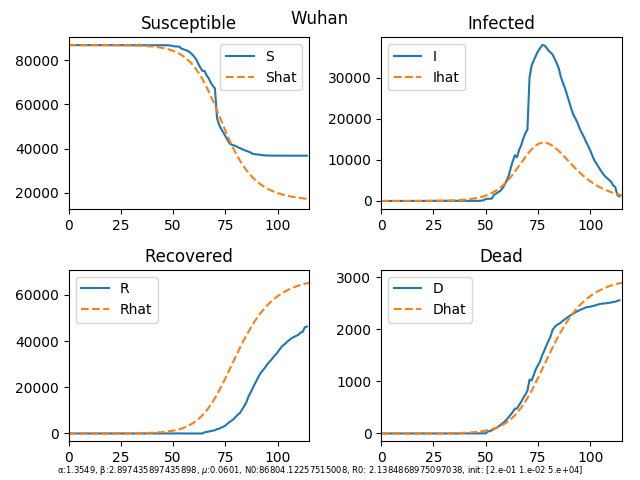
\includegraphics[width=9cm,height=9cm,keepaspectratio]{wuhan3.png}
  \caption{Estimated s, i, r, d from Wuhan epidemiological data. $R_0$ = 2.138}
  \label{fig:wuhan3}
\end{figure}
\vspace{-6mm}
Using initial guess $N_0 = 5x10^4$, the estimated $\alpha \approx 1.35 , \beta \approx 2.9, \mu \approx 0.06, N \approx 9x10^4$
\end{frame}

\begin{frame}
\begin{figure}
  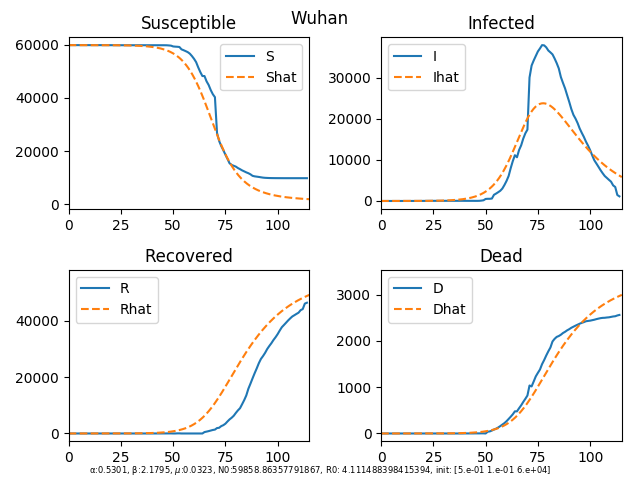
\includegraphics[width=9cm,height=9cm,keepaspectratio]{wuhan5.png}
  \caption{Estimated s, i, r, d from Wuhan epidemiological data. $R_0$ = 4.111}
  \label{fig:wuhan5}
\end{figure}
\vspace{-6mm}
Using initial guess $N_0 = 6x10^4$, the estimated $\alpha \approx 0.53 , \beta \approx 2.18, \mu \approx 0.03, N \approx 6x10^4$
\end{frame}
%Figure \ref{fig:boat1} shows a boat.
%\begin{figure}[h!]
%  \centering
%  \begin{subfigure}[b]{0.4\linewidth}
%    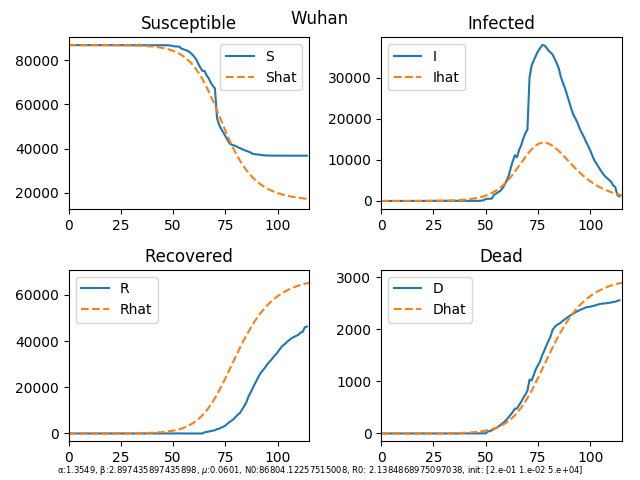
\includegraphics[width=\linewidth]{wuhan3.png}
%    \caption{Coffee.}
%  \end{subfigure}
%  \begin{subfigure}[b]{0.4\linewidth}
%   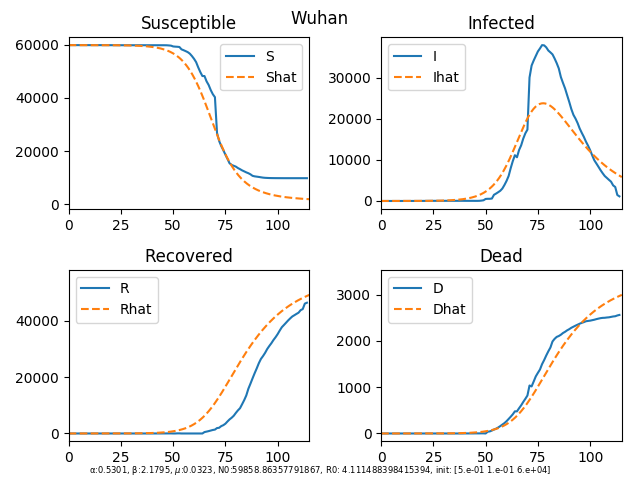
\includegraphics[width=\linewidth]{wuhan5.png}
%    \caption{More coffee.}
%  \end{subfigure}
%  \caption{The same cup of coffee. Two times.}
%  \label{fig:coffee}
%\end{figure}


%%%%%%%%%%%%%%%%%%%%%%%%%%%%%%%%%%%%%%%%

% All of the following is optional and typically not needed. 
\appendix
\section<presentation>*{\appendixname}
\subsection<presentation>*{Appendix}

\begin{frame}
  \frametitle<presentation>{Appendix}
    
  \begin{itemize}
  %\begin{thebibliography}{10}
    
  %\beamertemplatebookbibitems
  % Start with overview books.

  \item The code and data used for this project are published here: \href{https://github.com/NatashaTing/covid19-modelling}{Github/NatashaTing/covid19-modelling}.
 \end{itemize}
    
  %\end{thebibliography}
\end{frame}

\end{document}

